\documentclass{sigchi-ext}
% Please be sure that you have the dependencies (i.e., additional
% LaTeX packages) to compile this example.
\usepackage[T1]{fontenc}
\usepackage{textcomp}
\usepackage[scaled=.92]{helvet} % for proper fonts
\usepackage{graphicx} % for EPS use the graphics package instead
\usepackage{balance}  % for useful for balancing the last columns
\usepackage{booktabs} % for pretty table rules
\usepackage{ccicons}  % for Creative Commons citation icons
\usepackage{ragged2e} % for tighter hyphenation

% Some optional stuff you might like/need.
% \usepackage{marginnote} 
% \usepackage[shortlabels]{enumitem}
% \usepackage{paralist}
% \usepackage[utf8]{inputenc} % for a UTF8 editor only

%% EXAMPLE BEGIN -- HOW TO OVERRIDE THE DEFAULT COPYRIGHT STRIP --
% \copyrightinfo{Permission to make digital or hard copies of all or
% part of this work for personal or classroom use is granted without
% fee provided that copies are not made or distributed for profit or
% commercial advantage and that copies bear this notice and the full
% citation on the first page. Copyrights for components of this work
% owned by others than ACM must be honored. Abstracting with credit is
% permitted. To copy otherwise, or republish, to post on servers or to
% redistribute to lists, requires prior specific permission and/or a
% fee. Request permissions from permissions@acm.org.\\
% {\emph{CHI'14}}, April 26--May 1, 2014, Toronto, Canada. \\
% Copyright \copyright~2014 ACM ISBN/14/04...\$15.00. \\
% DOI string from ACM form confirmation}
%% EXAMPLE END

% Paper metadata (use plain text, for PDF inclusion and later
% re-using, if desired).  Use \emtpyauthor when submitting for review
% so you remain anonymous.
\def\plaintitle{Exploring Authoring of IoT Applications for Smart City Learning} \def\plainauthor{Francesco Gianni, Simone Mora, Monica Divitini}
\def\emptyauthor{}
\def\plainkeywords{Authors' choice; of terms; separated; by
  semicolons; include commas, within terms only; required.}
\def\plaingeneralterms{Documentation, Standardization}

\title{Exploring Authoring of IoT Applications for Smart City Learning}

\numberofauthors{3}
% Notice how author names are alternately typesetted to appear ordered
% in 2-column format; i.e., the first 4 autors on the first column and
% the other 4 auhors on the second column. Actually, it's up to you to
% strictly adhere to this author notation.
\author{%
  \alignauthor{%
    \textbf{Francesco Gianni}\\
    \affaddr{Norwegian Univesity of Science and Technology}\\
    \affaddr{Department of Computer and Information Science}\\
    \affaddr{Trondheim, Norway}\\
    \email{francesco.gianni@idi.ntnu.no} }\alignauthor{%
    \textbf{Simone Mora}\\
    \affaddr{Norwegian Univesity of Science and Technology}\\
    \affaddr{Department of Computer and Information Science}\\
    \affaddr{Trondheim, Norway}\\
    \email{simone.mora@idi.ntnu.no} } \vfil \alignauthor{%
    \textbf{Monica Divitini}\\
    \affaddr{Norwegian Univesity of Science and Technology}\\
    \affaddr{Department of Computer and Information Science}\\
    \affaddr{Trondheim, Norway}\\
    \email{monica.divitini@idi.ntnu.no} } }
    


% Make sure hyperref comes last of your loaded packages, to give it a
% fighting chance of not being over-written, since its job is to
% redefine many LaTeX commands.
\definecolor{linkColor}{RGB}{6,125,233}
\hypersetup{%
  pdftitle={\plaintitle},
%  pdfauthor={\plainauthor},
  pdfauthor={\emptyauthor},
  pdfkeywords={\plainkeywords},
  bookmarksnumbered,
  pdfstartview={FitH},
  colorlinks,
  citecolor=black,
  filecolor=black,
  linkcolor=black,
  urlcolor=linkColor,
  breaklinks=true,
}

% \reversemarginpar%

\begin{document}

\maketitle

% Uncomment to disable hyphenation (not recommended)
% https://twitter.com/anjirokhan/status/546046683331973120
\RaggedRight{} 

% Do not change the page size or page settings.
\begin{abstract}
Pervasive information visualization and interaction are fundamental tools to support learning in smart cities, for example to promote sustainable behaviors and social interaction. In this setting, information supporting learning goals is usually provided via screen-based interfaces such as public large displays and smart-phones. Those interfaces pose several usability issues and ignore the space of opportunities offered by research in tangible and embodied interaction.
Building on a review of existing work, we identify the main limitations of traditional approaches based on large displays and smart-phones apps, first from a technological point of view then connecting to implications for design, user interaction and experience.

In the paper we reflect on four implications related to the use of Smart Objects (SO) for smart city learning (SCL) applications: (i) Sensor data collection in the urban environment; (ii) Rich interaction techniques between users and technology; (iii) Background interaction and glanceable events in addition to foreground interaction for information display; (iv) Multimodal interaction, observable through different endpoints or objects distributed in the space.

We focus more in detail on new design opportunities, developing possible scenarios of interest that involve smart city learning.

\end{abstract}

\keywords{\plainkeywords}

\category{H.5.m}{Information interfaces and presentation (e.g.,
  HCI)}{Miscellaneous}\category{See}{\url{http://acm.org/about/class/1998/}}{for
  full list of ACM classifiers. This section is required.}

\section{Introduction}
Studies demonstrate that social connections in cities stimulates creativity and improves work quality \cite{florida_cities_2005}. This is only one of the reasons why the percentage of people living in urban environments is growing.

Smart cities present, by definition, a strong technological component.
In Technology Enhanced Learning (TEL), the role of technology is to direct, foster thinking and facilitate the acquisition of higher order skills \cite{goodyear_technologyenhanced_2010}.
Current research applied to learning in the cities seem to focus on two main technological means for learning contents: situated large displays and mobile devices, intended as tablets and smart-phones \cite{luff_mobility_1998}.

Traditional technology is a limiting factor: mobile devices and large screens support a very strict and confined set of interaction strategies. It's often not possible to tailor the user experience to properly fit the specific scenario because technology is too limiting.
Our goal is to design aiming at the best possible strategy for the users, building the technology around this process and avoiding the constraints typically introduced by more general-purpose hardware/software combinations.

We claim there is a space of opportunity for SCL applications in adopting novel ubiquitous computing approaches like tangible user interfaces (TUIs) and augmented objects (AOs). These technologies have already been found effective in supporting learning \cite{stanton_classroom_2001}, but their applications were mainly oriented to support learning as it happen in conventional schools and classrooms. The principal advantages in adopting these types of interfaces are (i) to enable the creation of rich and unobtrusive user experiences, (ii) to extend the type of data that can be captured to be used as learning content, including sensor data from the environment and from citizens' whereabouts. Therefore sensor-based TUIs could complement traditional approaches based on large screens and smartphones, especially when the learning environment can be as wide and heterogeneous as a city. Todays' increasingly adoption of sensors and IoT technologies are acting as enabling factors for the development of such interfaces; yet whether a number of studies have reported design guidelines for urban screens, there's a lack of guidelines to help the design of different types of interfaces.

As identified during a systematic mapping of the literature on smart city learning \cite{gianni_technologyenhanced_2016}, novel interaction modalities e.g. interactive objects and IoT, are not fully exploited. Even when used, the affordances employed are only a limited subset of the available ones. Unexplored opportunities emerged also when considering the learning aspect: rather than communities of citizens in the urban space, the research scenario usually involves schools or governance.

The need for more SCL research involving applications built around IoT and smart objects suggest the need to define a design space and a set of primitives, lying at different semantic levels, useful to structure and guide the authoring process.

%Toolkits play a role for facilitating the design and building prototypes of such applications.

% In this paper we...

%% ref toolkit




\section{Tangible user interfaces as a tool}
\subsection{Characteristics of Tangible Interfaces and Smart Objects}
Tangible user interfaces denote systems that rely on ``tangible manipulation, physical representation of data and embeddedness in the real space'', allowing for an embodied interaction with digital information. Embodied interaction, as defined by Dourish \cite{dourish_where_2004}, is a collection of trends emerged in HCI, relying on the common ground to provide a more natural user interaction with digital information.

Embodied interaction takes the interaction ``off the screen'' to the real world by distributing inputs and outputs in space rather than in time, desequentialising interaction and reducing the gap between where the information is created and where it is accessed. In this picture TUIs seamlessly integrate both representation and control of computation into physical artifacts: ``By treating the body of the device as part of the user interface -an embodied user interface- we can go beyond the manipulation of a GUI and allow the user to really directly manipulate an integrated physical-virtual device''.
When these artifacts also resemble and retain the functionalities of traditional objects, they can be called smart or augmented objects.

TUIs and smart objects (SOs) allow interaction designers to be free to experiment with new types of metaphors, taking advantage of the users' physical skills and providing interfaces which exploit people's knowledge with the everyday non-digital world.

End user development can also play an important role in this scenario \cite{lieberman_end-user_2006}. The focus is shifted on empowering users that are not familiar with any programming language, allowing them to develop and modify the original behavior of programmable systems.
End user development has gained interest even in connection with ubiquitous computing. Several works have explored the possibilities offered by end-users building applications for IoT and ubiquitous computing \cite{barricelli_designing_2015} \cite{bellucci_extreme_2015}.

% Unlike traditional ICT systems, the interactional paradigm is not one device per person. Rather, a single person interacts with a collection of devices that are orchestrated to expose coherent behaviours.

\section{Limitations of current technology}
\subsection{Smart City Learning}
The concept of smart-city has also been used in many different context and is associated with distinctive and innovative aspects that are often quite different. Big diversities are observed on the reasons \textit{why} different cities are defined as \textit{smart}.

This situation is the consequence of the lack of a clear and recognized definition of smart city.

Komninos \cite{komninos_intelligent_2002}, in his attempt to delineate the intelligent city, (perhaps the concept most closely related to the smart city), sees intelligent (smart) cities as ``\textit{territories with high capacity for learning and innovation, which is built\textendash in the creativity of their population, their institutions of knowledge creation, and their digital infrastructure for communication and knowledge management}''.

Smart cities are also a powerful ecosystem for learning. Smart city learning aim to support the improvement of all key factors contributing to the regional competitiveness: mobility, environment, people, quality of life and governance. The approach is aimed at optimizing resource consumption and saving time improving flows of people, goods and data\footnote{http://www.mifav.uniroma2.it/inevent/events/sclo/}.

Education in this context is pursued as a bottom-up process, where person and places are central. Smartness from a learning perspective exists both in the ambient data collected and among the communities that exists within a city.

The separation between student and teacher will fade out. Their role will be content or situation dependent: everybody will be a learner and the relation between persons will get a bigger role.


\subsection{Characteristics of Smart City Learning Applications}

%%...what are smart city learning applications?
%%...what kind of learning and what learning goals?

Technologies like mobile devices, tags, web based applications, geographical information and e-learning systems have already been used to develop smart city learning applications on the field \cite{perez-sanagustin_multichannel_2013} \cite{delfatto_geographic_2013}.

%%%%%%
Smart city learning applications consist in the implementation of urban informatics techniques and approaches to promote innovative engagement strategies \cite{amayocaldwell_urban_2013}.
Studies found that urban informatics provide an innovative opportunity to enrich students' place of learning within the city \cite{amayocaldwell_urban_2013}.

No doubt that among the consequences of such attention there is an acceleration in supporting the integration and embedding of ICT within physical environments to realize what has been defined the \textit{everyware} \cite{giffinger_smart_2007}.

% Other studies focused on the transformation from a \textit{space} of learning to a \textit{place} of learning in the smart city context, this is achieved through the exposure of real world urban sites and issues\cite{amayocaldwell_urban_2013}.



\section{Augmented objects and TUIs for SCL applications}
We identified a list of primitives at different semantic levels useful to describe, design and author applications for SCL supported by SOs and TUIs:

\begin{figure}[htb]
\centering
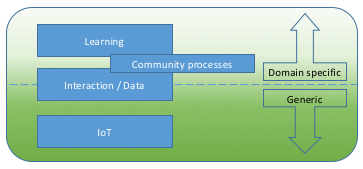
\includegraphics[width=8cm]{img/primitive_layers}
\caption{Semantic layers of the primitives.}
\label{fig:layers}
\end{figure}


\subsection{Generic level}
\medskip

\subsubsection{PHYSICAL MANIPULATION}
\begin{description}
\item [Touch] as the ability to detect interactions like a simple touch, swipes, multiple taps et simila;
\item [Multi-axial rotation] detects with sufficient precision object rotation and tilt;
\item [Shake and displacement] intended as the ability to detect when the object is shaken vigorously or is being physically moved.
\end{description}

\subsubsection{FEEDBACK AND OUTPUT}
\begin{description}
\item [Led light] can be used as a low fidelity output, more complex communication strategies can be implemented, like blinking, color fading and led matrix;
\item [Haptic] defined as vibration pattern that differ in intensity and duration;
\item [Sound] intended as simple beeping or composition of multi-tone sounds.
\end{description}

\subsubsection{OBJECT AUGMENTATION}
\begin{description}
\item [Untethered operation] augmented object should work independently and autonomously, without being hooked to any external device that provides connectivity or power support;
\item [Easily embeddable] technology should be easy to integrate into objects, without altering the original function and nature of the object;
\item [Energy autonomous] the objects should be as much autonomous as possible, effective energy usage, battery efficiency and energy harvesting can help at this regard.
\end{description}


\subsection{``Generic/Domain Specific'' overlapping level}
\medskip

\subsubsection{DATA}
\begin{description}
\item [Sensor data collection] intended as the opportunity to employ data gathered in real time from the surrounding ambient. Domain specific data can include for example air pollution, geolocation, temperature;
\item [Data visualization] as the ability to support visualization of simple information through low fidelity output. Adapting to the domain implies that only a specific subset of data visualization strategies are suitable. It is also important to trigger the learning process and help the users reflect on their experience;
\item [Data processing] involves elaboration of data coming from sensors and/or from third party services.
\end{description}

\subsubsection{INTERACTION STRATEGIES}
\begin{description}
\item [Object sharing] intended more as a dimension, SOs allow to freely move from the private and personal sphere to sharable artifacts and community objects, continuously exploring the space in between;
\item [Background/foreground] interaction should be possible when the object is in the center of attention, but also when in background, providing context information possibly through glances and nudging;
\item [Distributed] interaction with several augmented objects orchestrated as a single user interface;
\item [Multimodal] object interaction based on more than one strategy, e.g. touch and speech recognition on the same object;
\item [Sensor based] it's an enabler for physical manipulation, since smart objects do not provide a dedicated interaction interface (like a keyboard or buttons), the interaction happens with the object itself.
\end{description}


\subsection{Domain Specific level}
\medskip

\subsubsection{LEARNING}
\begin{description}
\item [Reflection] occurs when reflecting on previous experience and behaviours;
\item [Behaviour change] the explicit goal is to modify or improve a specific behaviour;
\item [Data enabled] knowledge is extracted directly from collected data;
\item [Social] occurs when it's the result of a community process;
\item [Game based] process gamification and situated games where smart objects extend and improve the gameplay and the learning experience.
\end{description}

\subsection{Challenges}
Although the need for a set of authoring primitives is driven by the possibility to follow a more lightweight design approach and to better adapt to the context, defining an appropriate semantic level can be intricate since it is closely related to the skills of the target group (end-users, developers, designers, etc).
A series of challenges are also connected to the authoring process:

\begin{itemize}
    \item Several semantic levels require several competencies, which implies that collaboration among experts is fundamental to address complexity along multiple dimensions;
    \item Proposed primitives can be combined in multiple ways, picking the best alternatives for each application can still be challenging;
    \item Data are a valuable source of knowledge to improve the design process, analytics are important to keep track of the process and spot opportunities for improvements;
    \item The learning process can follow several approaches. Based on the specific domain, can be challenging to find the most effective;
    \item Promoting creativity is essential when dealing with different target groups, it is important to balance and define the primitives in a way that are useful to guide the design without introducing heavy constraints that can hinder creativity and original solutions.
\end{itemize}

\subsection{Examples of applications}
Example of SCL applications resulting from this approach can be situated augmented games where players interact with smart pones that are also location aware. Pones can be displaced in the environment, shared between players, can guide the gameplay, support different interaction modalities and provide simple triggers for reflection, supporting the learning experience.

Another example can involve the use of augmented objects to facilitate cooperation between communities in the city. The process of urban planning in Norway require the municipalities to gather feedback from communities of citizens.
Difficulties has been encountered in providing value in the process, since traditional methods do not fit well when dealing with children for example.
Using smart objects that can be physically manipulated and provide an engaging experience can motivate and attract participants to collaborate and at the same time stimulate their creativity.

\subsection{TILES toolkit for AOs}
Tiles is a rapid prototyping toolkit for AOs, it is composed by: (i) a set of abstracted physical interaction primitives and composition rules, (ii) hardware modules with sensors and actuators to generate and consume primitives, (iii) a software framework to allow manipulation and use of primitives within a specific application logic. TILES toolbox aim at supporting the iterative process of building prototypes of interactive objects, using abstract primitives developed as a bridge to gracefully support the transition between design and implementation steps. Prototypes might then be released for user testing.

TILES is a promising project that fits very well with the generic authoring primitives defined above. It is designed taking into account many of the challenges usually found in prototyping toolkits.
TILES' flexible software framework and event-driven messaging system allow to develop abstractions at different semantic levels for the coding process. This helps to match more closely the skills of end users, developer, designers and possibly other categories.

\section{Conclusion}
In this article we proposed a new way to empower technology in SCL scenarios. Starting from the literature, the limitations of current technological patterns were highlighted, then AOs and TUIs were introduced as a viable alternative to more traditional approaches. TILES is then proposed as a valuable toolkit for rapid prototyping with SOs.

Our claim is that the proposed primitives can be combined and used to author and design SCL applications that empower SOs, IoT and TUIs. Strengths and challenges of the authoring process were also presented.

Using this approach we believe it will be possible to successfully address several of the challenges that characterize research and interaction in SCL scenarios. More research and feedback are needed to better ground the claims proposed.


\balance{} 

\bibliographystyle{SIGCHI-Reference-Format}
\bibliography{bib_avi}

\end{document}

%%% Local Variables:
%%% mode: latex
%%% TeX-master: t
%%% End:
